\def\be{\begin{equation}}
\def\ee{\end{equation}}

\newcommand{\nucl}[3]{ \ensuremath{ \phantom{\ensuremath{^{1}_{#2}}} \llap{\ensuremath{^{#1}}} \llap{\ensuremath{_{\rule{0pt}{.75em}#2}}} \mbox{#3} } }





\documentclass[12pt]{article}
\usepackage{graphicx}
\usepackage{notoccite}
\usepackage{epigraph} % epigraph
\usepackage{float}
\usepackage[hyphens]{url}
\usepackage[square, numbers, comma, sort&compress]{natbib}  % Use the "Natbib" style for the references in the Bibliography
\usepackage{verbatim,listings}  % Needed for the "comment" environment to make LaTeX comments
\usepackage{array}  % Needed for the "comment" environment to make LaTeX comments
\usepackage{vector}  % Allows "\bvec{}" and "\buvec{}" for "blackboard" style bold vectors in maths

% \documentclass[a4paper,12pt]{article}
%\usepackage[a4paper,vmargin={20mm,20mm},hmargin={20mm,20mm}]{geometry}
\usepackage{amsmath,amsfonts,amsthm,color,psfrag,epsf,graphicx}
% \usepackage{pstricks}
\usepackage{enumerate,caption}
%\usepackage[lined,algonl,boxed]{algorithm2e}
\usepackage[ruled,linesnumbered,vlined]{algorithm2e}
\usepackage{float}
% \SpecialCoor
\def\subsum{\mathit{\Sigma}}




\def\ifthesis{\iftrue}
\setcounter{secnumdepth}{2}
\newenvironment{myindentpar}[1]%
{\begin{list}{}%
		{\setlength{\leftmargin}{#1}}%
		\item[]%
	}
	{\end{list}}




\graphicspath{{Figures/}}  % Location of the graphics files (set up for graphics to be in PDF format)
\usepackage{epigraph} % epigraph
%customize: \setlength{\epigraphwidth}{7cm}\setlength{\epigraphrule}{0pt}
%use: \epigraph{text}{reference}

%customize: \setlength{\epigraphwidth}{7cm}\setlength{\epigraphrule}{0pt}
%use: \epigraph{text}{reference}
\begin{document}
\bibliographystyle{unsrt}
%\section*{Declaration}
%Figures .... and the accompanying discussion have previously been published in . 
\section{Introduction}

As detailed in Chapter X, ball-pen probes have been successfully implemented in fusion plasmas to make measurements of the plasma potential and electron temperature. These plasmas are characterised by high temperatures, high densities and strong magnetic fields. BPPs have also been implemented in low temperature, low density and slightly magnetised plasmas \cite{alow_temp}, \cite{low_t} \cite{mirabelle}. These plasmas are useful in various technological applications such as plasma etching. In \cite{mirabelle}, a BPP was used  in helium and argon plasmas at pressures in the $10^{-2}$ Pa range, with an electron density of $10^{16} - 10^{17}$ $m^{-3}$, an electron temperature of $1-7$ eV and various magnetic field strengths up to a maximum of 80 mT. Three BPPs of inner diameter $1$, $0.6$ and $0.3$ mm were tested and compared to measurements of the plasma potential made by an emissive probe. It was found that the floating potential measurement made by the larger probes increasingly deviated from the plasma potential as the magnetic field strength was increased, with the probe floating negatively with respect to the plasma potential. However, the smaller probe was capable of measuring the plasma potential across the range of field strengths. In these plasma conditions, the electrons are magnetised but the ions are unmagnetised which is a different regime from a tokamak plasma in which both species are magnetised. The BPP in this plasma was insensitive to the ion gyroradius, its capability to measure the plasma potential was determined by its ability to effectively screen out the electron current. In regimes where the tunnel diameter was smaller than the electron Larmor radius, drifting electrons would hit the tunnel wall before making it down to the collector thus reducing the perpendicular electron flux. For this reason, the $0.3$ mm probe was still capable of operating as a BPP at $80$ mT whilst the larger probes exceeded the size of the electron Larmor orbit and could not screen out the electron current. In \cite{low_t}, three BPPs with tunnel diameters ranging between $1.5-2$ mm were installed on a magnetron device filled with an argon plasma of density $\approx 1 \, \times \, 10^{16} \, m^{-3}$. In the experiments, the electron temperature ranged from $0.9-3.4$ eV, the pressure ranged from $1-20$ Pa and the field strength from $20-40$ mT. The work found a limit of applicability for use of the BPP in low temperature plasmas. The probe was found to float around the plasma potential provided the ratio of magnetic field strength to pressure exceeded $10$ mT/Pa. Below this value, the electrons are not sufficiently magnetised and can travel to the probe collector unimpeded, the BPP collector then floated at the same potential as a standard Langmuir probe, regardless of the collector recession depth. In both papers the ions were unmagnetised and so the BPPs were insensitive to the gyromotion of the ions. In our work we extend the investigation of the applicability of BPPs in low temperature plasmas, to field strengths found in tokamaks, in regimes where both charged species are magnetised.


The results presented in this chapter were obtained from experiments performed in the system illustrated in figure \ref{fig:rig}. The system consisted of an aluminium chamber with a cross sectional area of $14$ $cm^2$ and $7.5$ cm deep. The system generated a radio-frequency (RF), argon plasma at 13.56 MHz in a parallel plate capacitively coupled cell. The electrodes, 4 cm in diameter were spaced 4 cm apart. The plasma is powered by a Dressler Cesar 136 coupled through a matching unit to the powered electrode. A Helmholtz coil is used to generate the magnetic field uniformly (within $2\%$) throughout the plasma. The plasma density was $\approx$ $10^{15}$ $m^{-3}$ and the electron temperature was $3$ eV. 


\begin{figure}[H]
\centering
\includegraphics[width=1.0\textwidth]{ChamberSchematic4.jpg}
\caption{Schematic of the experimental system equipped with a mass flow controller (MFC), a matching unit (MU), a current sensor (Ip) and a voltage probe (Vp). The plasma was diagnosed with a ball-pen probe (BPP) and an emissive probe.}
\label{fig:rig}
\end{figure}

%T	inves-ga-on	of	the	effect	of	different	recession	depths,	are	compared	to	an	emissive	probe	

In this experiment, four BPP designs were investigated under various magnetic field strengths, from $0 - 0.5$ T. Two collector diameters of 2 mm and 4 mm  were investigated, with the outer diameter of the tunnel being 3 mm and 5 mm respectively. For each diameter, experiments were carried out with a flat collector design and a tapered, conical collector design allowing the effect of varying the size of the collector area and it's shape to be studied. The BPP collectors were made of stainless steel and mounted on a retractable arm so that the effect of recession height could be studied. The tunnel was formed of aluminium oxide, an insulating material. The BPPs could be operated in floating mode or biased to extract an I-V characteristic. In order to obtain accurate values of the floating potential, a high impedance circuit was required, this is discussed further in section \ref{Sec:impedance}. I-V characteristics were obtained by connecting the collector to a Hiden unit. The Hiden unit used was the ESPION Advanced Langmuir Probe, Model EPIU. ESPsoft Version 7.2 was used to communicate to the unit to generate the IV curves. The floating potential measurements of the BPPs are compared to the plasma potential measurements inferred from the emissive probe, over a range of plasma pressures and powers.  The emissive probe consisted of a thoriated tungsten wire, $25$ $\mu m$ in diameter and 1 cm long. The electrical arrangement for the emissive probe and the underlying theory behind its operation is discussed in section \ref{sec:emissive}.  The chapter then moves on to explain the need for high impedance circuity to make accurate floating potential measurements in a low temperature plasma. Results for each of the BPP collectors and the emissive probe are then discussed.   





%Did we do something to check RF compensation wasn't required
%
%
%% Between the two end connectors
%%of the probe stem there was a total measured impedance of
%2 '. %Heating of the wire was achieved by passing a 50 Hz ac current through it, tapped off from the mains supply via a variable transformer and a fixed transformer.
%
%What was the technique to get the data, Paul mentioned it was refined 
%
%
%
%
%
% When h < 0, the impedance
%between the probe and the plasma is significantly increased
%and can reach several hundred M	. To avoid leakage current,
%an AD549 electrometer amplifier with a high impedance
%(1015 	) is used as a unit gain follower for electrostatic potential
%measurements
%
%The ball-pen probe was constructed in a way that enabled the movement/shift of the collector. 
%
%What was our ball pen made from? 
%
%Floating potential measured using high impedance circuit op-amp 
%
%IV curves obtained using Hiden, model number?
%
%Thickness and material of emissive probe?  
%
%What was the radius of collector and outer radius of each tunnel? 
%
%Which Op-Amp did we use, did we use the same voltage follower circuit as  http://aip.scitation.org/doi/pdf/10.1063/1.4916572 ?  
%
%Can we get Vfloat from IV characteristic and float to compare the two? 
%
%
%. For Te comparable with the temperature Tw of
%emitted electrons (temperature of the emissive probe wire),
%the floating potential of the emissive probe might overestimate
%the plasma potential;  7A. Marek, M. Jılek, I. Pickova, P. Kudrna, M. Tichy, R. Schrittwieser, and
%C. Ionita, Contrib. Plasma Phys. 48, 491 (2008).
%0
%
%
%Talk about operating in regimes where no species are magnetised, then the electrons then both 
%
%explain the simulation, used real mass, real temperatures, real dimensions, allowed by low density of plasma 
%
%
%in http://aip.scitation.org/doi/pdf/10.1063/1.4916572 they found the BPP only operated as a BPP once B/p > 10mT/Pa do we find this as well?
%
%
%
%
%The neutral gas pressure in tokamaks is very low, and
%the electron motion is therefore clearly influenced mostly by
%the magnetic field. In order to take into account the effect of
%the neutral gas pressure that is usually higher in lowtemperature
%plasma devices,
%
%Introduce the experimental set up - RF plasmas
%Low temp argon plasma   0.25eV ions approx 3 eV electrons various field strengths up to 0.5T.  
%Used emissive probe and ball pen probe 
%Emissive probes used to measure plasma potential in RF plasmas  and tokamaks cite 
%E. Y. Wang, N. Hershkowitz, T. Intrator, and C. Forest, Rev. Sci. Instrum.
%57, 2425 (1986). 
%
%2
%R. Schrittwieser, J. Adamek, P. Balan, M. Hron, C. Ionita, K. Jakubka,
%L. Kryska, E. Martines, J. Stockel, M. Tichy, and G. Van Oost, Plasma
%Phys. Controlled Fusion 44, 567 (2002).  
%
%At critical emission the presheath drop is
%approximately 0.8Te/e,
%10 so, ultimately, the potential difference
%between the floating surface and the bulk plasma
%(VF  VP) is
%$VF  - VP \approx - 1.8Te$
%
%Did we see higher potential drops for emissive than BPP? 
%
%For BPP we know alpha is roughly 0.6. For emissive it is saying alpha is 0.95Te so BPP should give closer measurement
%
%http://w3.pppl.gov/~fisch/fischpapers/2011/Sheehan.POP.2011.pdf
%
%
%Due to low temps, use of emissive probe was possible 
%
%Talk of using high impedence 
%
%
%Before presenting the results it is useful to review the emissive probe theory.  

\section{Emissive Probe Theory}
\label{sec:emissive}
The emissive probe is another advanced probe technique designed to measure the plasma potential directly. The underlying principle of both the BPP and the emissive probe is to balance the magnitudes of the ion and electron saturation currents. If these two quantities are equal, the probe will float at the plasma potential. Unlike the BPP that aims to reduce the magnitude of the electron saturation current, the emissive probe instead enhances the ion saturation current. The emissive probe consists of a thin filament of wire that is heated, causing it to emit electrons. If the probe is biased negatively with respect to the plasma potential, the electrons escape the probe surface and travel into the plasma. In terms of current to the probe, an electron emitted is the same as an ion collected, so the emitted electrons enhance the ion current to the probe. If the probe is biased more positively than the plasma potential only the high energy tail of the electrons can escape into the plasma. An I-V characteristic for a heated emissive probe then consists of the ion current and both the emitted and collected electron currents. The collected electron current is the same as that of a standard probe 



\begin{equation}
 I_e (V_{probe}) =    \begin{cases}
   I_e \exp \left (\frac{-e(V_p - V_{probe})}{T_e} \right), & \text{if $v_{probe} < v_p$}.\\
    I_e^{sat} & \text{if $V_{probe} \geq v_p$}.
  \end{cases}
\end{equation}


The emitted current ($I_{e0}$) is given by 


\begin{equation}
 I_{e0} (V_{probe}) =    \begin{cases}
   I_{e0}  & \text{if $v_{probe} \leq v_p$}.\\
      I_{e0} \exp \left (\frac{-e(V_p - V_{probe})}{T_{probe}} \right), & \text{if $V_{probe} \geq v_p$}.
  \end{cases}
\end{equation}
At biases less than the plasma potential, at a constant emissive probe temperature ($T_{probe}$), the emission current is constant and equal to $I_{e0}$, where $I_{e0}$ is the temperature limited current given by the Richardson-Dushman equation \cite{emissionya}

\be 
I_{e0} = A {T_{probe}}^2 S \exp \left( \frac{e \phi_w}{T_{probe}} \right)
\ee where $A$ is the Richardson constant , $\phi_w$ is the work function of the metal and $S$ is the surface area of the wire. In this regime, the emission of electrons is limited by the temperature of the wire, so this regime is known as the temperature limited regime.

A significant flux of emitted electrons can change the sheath structure around the probe leading to a reduction of the floating potential and an effect on the shape of the I-V characteristic around the plasma potential. These space-charge effects need to be taken into account if the correct plasma potential is to be obtained from the I-V curve of an emissive probe. Various methods have been developed to extract $V_{plasma}$, of these the inflection point in the limit of zero emission method is regarded to most accurately measure the plasma potential \cite{embest}. For the inflection point in the limit of zero emission method, inflection points in the I-V curve are measured for the probe at various low emission levels, such that the temperature limited emission current is on the order of the electron saturation current or less. The potential of these inflection points is then plotted against emission current producing a linear plot which is then extrapolated to zero emission to obtain the plasma potential \cite{inflection}. In the presence of strong magnetic fields, the I-V curve in the electron collection region is distorted and the inflection point can be hard to determine \cite{inflection}. As a result, an alternative method for measuring the plasma potential was required. It is known that as an emissive probe is heated, the floating potential of the probe rises as the emission increases, rising rapidly at first and then plateauing at a potential deemed to be the plasma potential \cite{review_em}, \cite{bradley}. This is known as the floating point in the limit of large emission method and was used to obtain the following emissive probe results presented in this chapter. 

The electrical arrangement for the emissive probe is shown in figure \ref{fig:emissive}. The probe wire was looped into a semicircle and then fitted into the probe stem. The wire was heated by passing a 50 Hz ac current through it. 
\begin{figure}[H]
\centering
\includegraphics[width=1.0\textwidth, height = 8cm]{em_circuit.png}
\caption{Schematic of the circuit used to heat the emissive probe and measure the floating potential.}
\label{fig:emissive}
\end{figure}

%UPDATE EMISSIVE PROBE CIRCUIT
%This method is similar to the way the plasma potential is found from a standard collecting Langmuir probe in which taking the derivative of the I-V curve reveals an inflection point at the plasma potential. Data from a Langmuir probe is often noisy, taking derivatives of the data amplifies the noise which is the source of a large error in the inferred plasma potential. For an emissive probe, I-V curves can be obtained at different heating powers. Due to space charge effects, the inflection point of these curves is shifted to a negative potential relative to the plasma potential. The extent of this shift has a linear dependence with emission levels \cite{inflection}. The inflection point will only be at the plasma potential for the case of zero emission. For the inflection point in the limit of zero emission method, inflection points are measured for the probe at various low emission levels, such that the temperature limited emission current is on the order of the electron saturation current or less. The potential of these inflection points is then plotted against emission current producing a linear plot which is then extrapolated to zero emission to obtain the plasma potential. This method has the advantage of using numerous inflection points to obtain the plasma potential, providing a more accurate measurement than that of a single collecting probe. Stated measurements of the plasma potential from the emissive probe were obtained using this method.

%Actually inflection method hasn't really be used in or results we used the Floating point in the limit of large
%emission method, inflection is problematic in strong magnetic fields  Sheehan and N. Hershkowitz, “Topical review: Emissive probes,” Plasma
%Sources Sci. Technol., vol. 20, p. 063001, 2011. and  J. Smith, N. Hershkowitz, and P. Coakley, “Inflection point method of interpreting
%emissive probe characteristics,” Rev. Sci. Instrum., vol. 50, p. 210,
%1979 

%CHANGE TO FLOATING POTENTIAL METHOD, just briefly describe other method and say its not suitable for magnetic fields can add the other plot from poster then conclusions




\section{High Impedance Circuit for Ball-Pen Probe Floating Potential Measurements} 
When measuring the floating potential of a probe, the probe can be considered as the voltage source ($V_S$) in the following circuit:  

\begin{figure}[H]
\centering
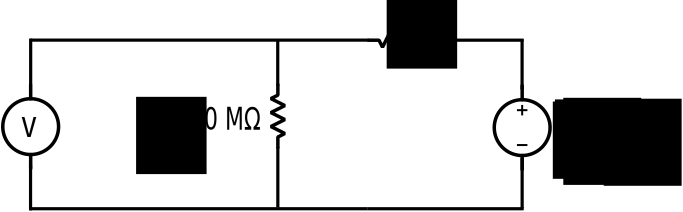
\includegraphics[width=1.0\textwidth]{basic_circuit.pdf}
\caption{Representation of the probe circuit to measure the floating potential.}
\label{fig:emissive}
\end{figure}

The potential difference is measured by a voltage probe with a resistance of 10 M$\Omega$. The other source of resistance in the circuit is $R_S$ which represents the impedance between the probe and the plasma and is an unknown quantity. For a standard Langmuir probe, $R_S << R_{in}$  therefore most of the potential drop occurs across $R_{in}$ and the voltage probe is able to measure $V_S$. However, for a BPP with a recessed collector, particle collection to the probe is not due to motion parallel to the magnetic field, it relies on cross-field motion. This greatly increases the effective impedance of the BPP. As a result, the potential drop does not occur entirely across $R_{in}$ and as the value of $R_S$ is not known, its effect can not be factored out. By adding an additional resistor into the circuit ($R_2$), with a high impedance to form a potential divider, the effect of the BPP's high impedance can be negated.  

\begin{figure}[H]
\centering
\includegraphics[width=1.0\textwidth]{divider_circuit.pdf}
\caption{A potential divider is used to determine the correct floating potential of the probe.}
\label{fig:emissive}
\end{figure}

Provided $R_2 >> R_S$, $V_S$ can be determined from the reading on the voltage probe ($V_{out}$). 
\begin{equation}
V_S = V_{out} \frac{(R_2+ R_{in})}{R_{in}} 
\end{equation}
Once the collector is recessed inside the BPP tunnel, the impedance can rise to several hundred M$\Omega$ \cite{mirabelle}. Therefore, $R_2$ must have a very high impedance. Figure \ref{fig:increasing_R} shows the floating potential measured by the voltage probe as the value of $R_2$ is increased. Even for impedance values as high as $700$ M$\Omega$, the effect of the probe impedance is still evident and hence the value of $V_f$  has yet to saturate. In order to obtain sufficient impedance, $R_2$ was replaced with a voltage follower using the operational amplifier OPA452T by Texas Instruments that had a high input impedance of $10^{13}$ $\Omega$. This operational amplifier has previously been used in \cite{low_t} to make direct floating potential measurements of a BPP in a low temperature plasma. The voltage follower circuit is show in figure \ref{fig:follow}. 




\begin{figure}[H]
\centering
\includegraphics[width=1.0\textwidth, height = 7cm]{increasing_R.pdf}
\caption{The measured value of the BPP floating potential with increasing resistance of $R_2$ in the potential divider circuit. As $R_2$ increases so does the measured floating potential. }
\label{fig:increasing_R}
\end{figure}


\begin{figure}[H]
\centering
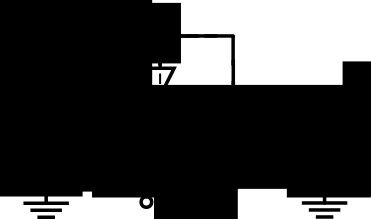
\includegraphics[width=1.0\textwidth, height = 8cm]{op_amp.pdf}
\caption{The voltage follower circuit used to provide high impedance in the potential divider circuit. }
\label{fig:follow}
\end{figure}


%Emissive probes have an exponential region that depends on the probe temperature rather than the plasma temperature and as $T_e >> T_{probe}$ emissive probes can measure a potential closer to the plasma potential. 
%Plasma potential from emissive probes can be obtained in multiple ways. WE used the floating potential with large emission method. 



\section{Results}
Initial experiments were carried out with a Langmuir probe in place of the BPP in order to check the validity of the emissive probe plasma potential measurements for a range of plasma powers and pressures. The Langmuir probe wire in these experiments was 1 cm long and with a diameter of $25$ $\mu m$. Plasma potentials from the Langmuir probe were derived from the inflection point of the I-V characteristics. Derived values of the plasma potential for both probes is shown in figure \ref{fig:emVSlp}. In these comparison runs the plasma was unmagnetised. Magnetising the plasma distorts the electron collection region of the Langmuir probe I-V curve, increasing the noise in the inflection point measurement.

\begin{figure}[H]
\centering
\includegraphics[width=1.0\textwidth, height = 10cm]{emVSlp.png}
\caption{The plasma potential as measured by the emissive probe and the Langmuir probe for a variety of plasma powers and pressures.}
\label{fig:emVSlp}
\end{figure}
The plasma potential measurements from both probes agree within 3 eV which is approximately the electron temperature, this suggests the floating point method is valid. The emissive probe measurement should remain valid in magnetised plasma up to 250 mT, after which the Larmor radius becomes smaller than the diameter of the emissive wire. 

%Can we get a Te from langmuir probe data? 

%Can we get a comparison of floating potential measured by BPP directly and from IV curve to show the op-amp works?
The capability of the BPP to make plasma potential measurements for a range of magnetic field strengths was tested for each collector. For each experiment the plasma power and pressure were held constant as was the field strength. The collector began fully recessed inside the tunnel at $h = - 10$ mm and was then moved forward in increments with a new value for $V_f$ recorded at each position. After the final reading was taken at $h = 5$ mm, the magnets were turned off to allow them to cool. The collector was then fully recessed before beginning the investigation under a new field strength. Shown in figure \ref{fig:fieldInvest} are the results obtained from the 2 mm tapered collector. The pressure was 0.45 Pa and the power was 10 W.


\begin{figure}[H]
\centering
\includegraphics[width=1.0\textwidth, height = 10cm]{field_investigation.png}
\caption{The floating potential of the 2 mm tapered BPP collector as a function of recession depth for different field strengths. }
\label{fig:fieldInvest}
\end{figure}

In the unmagnetised plasma the probe does not operate as a BPP. Once the collector is recessed inside the tunnel there is a decrease in the floating potential and little variation with further recession. The probe is also unable to operate successfully for the low field runs. In this regime the electrons are magnetised but the ions are not. The electron Larmor orbit is approximately 0.5 mm for the 8 mT case, the tunnel diameter is then 4 $\rho_e$ and so the probe is unable to effectively screen out the electron current to the collector. The probe begins to exhibit BPP behaviour on increasing the field strength to $81$ mT. Now the ions as well as the electrons are magnetised. The collector potential begins to climb as the collector is recessed, reaching a peak potential at $\approx 25$ V for the three high field strengths. The 81 mT case shows a large plateau region in which there is little variation of the floating potential with probe recession. The length of this plateau region decreases with increasing field strength. As discussed in Chapter X, in order for ions to reach the collector their motion around the field must bring them to the collector before their parallel motion brings them to a tunnel wall, their perpendicular motion is assisted by E x B drifts. As the field strength increases, the Larmor radius decreases. Once the probe is recessed beyond $\approx 10\rho_i$ only a limited portion of the ion population current can reach the collector, the collector then floats more negatively to repel electrons which are still capable of reaching it by E x B drift motion and reflecting off the sheaths of the tunnel wall. It would appear that the depth of the collector is an important design constraint in strongly magnetised, low temperature plasmas where the Larmor radius of the ions is much smaller than that of an ion in a fusion plasma. The probe depth is not an important parameter for the intermediate 81 mT case. 

The experiment was then repeated for the 2 mm flat collector. The plasma had to be switched off so that the new collector could be inserted into the vacuum chamber. As a result, the plasma conditions may vary for the different collectors, although both were operated at the same power and pressure. Figure \ref{fig:pressure} shows the results of the identical experiment with the flat collector as well as the results under a higher operating pressure of 9.6 Pa.  


\begin{figure}[H]
	\setbox0\hbox{%
		\includegraphics[width=.5\textwidth]{flat_low_pressure.png}%
	}%
	\setbox2\hbox{%
		%\includegraphics[width=.5\textwidth]{top_down.pdf}%
		\includegraphics[width=.5\textwidth]{flat_high_pressure.png}%
	}%
	
	\noindent
	\parbox{.5\textwidth}{%
		\centering
		\unhbox0
		
	}%
	\hfil
	\parbox{.5\textwidth}{%
		\centering
		\unhbox2
		
	}%
	
	\caption{The floating potential of the 2 mm flat BPP collector as a function of recession depth for different field strengths. The plasma pressure was 0.45 Pa and 9.6 Pa for the left and right plots respectively.}
	\label{fig:pressure}
\end{figure}
%At field strengths below $81$ mT the probe is unable to operate as a BPP. 
%
%Took 81mT slightly deeper before reching plasma potential
%
%$2mm tapered one, doesn't work for intermediate field strengths, need to be at least 81 mt$. Does it not work at weaker field strengths because electrons aren't sufficiently confined? 
%$8mt doesn't work for the 0.45 Pa case, so 10mT/Pa$ isn't the only definining feature. At this field strength what is the extent of magnetisation for both species? This is like the other BPP where probe size became important, in these low field cases only the electrons are magnetised, the BPP can only effectively screen the electron current if the probe is the same size as the larmor radius. Our probes are much larger than $R_l$ electron so they can't measure the plasma potential for any low magnetisation values. Once both species become magnetised we are then in the fusion regime and the probe can operate as a BPP. 
%Potential for the stronger fields drops off more quickly, ion larmor radius becomes too small for ions to reach bottom of probe?  Floating potential of probe otuside tunnel changes with fields strength, does this correspond to values with see with emissive probe, i.e if plasma potential changes then changing floating potential also makes sense 
%
%Say that the low fields probe basically floats at some potential as standard LP

For the low pressure run, the flat collector exhibits the same behaviour as the tapered collector, only operating as a BPP once the ions become magnetised. The 81 mT case again has the largest plateau region. However, higher magnetic field strengths are required to maintain BPP behaviour once the pressure is increased to 9.6 Pa. In a fusion plasma the neutral gas pressure is on the order of $10^{-6}$ Pa and the effect of collisions on charged particle motion in the BPP tunnel can be neglected. However, at high neutral pressures, the ions undergo multiple collisions in a gyro-orbit destroying their magnetisation. The 81 mT case falls short of the minimum 10 mT/Pa required for the probe to operate as a BPP \cite{low_T} which reduces the peak floating potential. 
Particle-In-Cell simulations of the 2 mm flat collector were carried out using the model introduced in Chapter X. The reduction in plasma density of more than a factor of 100 from the MAST SOL enabled the use of much larger grid cells and therefore larger probe depths could be explored. For these runs, singly charged ions were assumed with realistic ion masses. The simulation parameters are given in table \ref{tab:sim_parameters}. Two sets of simulations were carried out, an unmagnetised set and a magnetised set in which the magnetic field strength was set to 250 mT. The probe was operated in floating mode in these simulations and the plasma potential was set to 25 V. Collisions are neglected in the simulations. The results of these simulations are shown in figure \ref{fig:sim_results}.
\begin{table}[]
	\centering

	\begin{tabular}{c|c|c}  %{lllll}
		 &  &  \\ % \\ \hline 
		Magnetic field strength $B$             & 0 T or 0.25 T                                               \\
		Magnetic field inclination $\theta$                & $10^{\circ} $      \\
		Plasma density $n$               & $1.\, \times \, 10^{15} \, m^{-3}$ \\ 
		Electron temperature $T_e$ &      $ 3$ eV     \\ 
		Ion temperature  $T_i$ &     $0.025$ eV  \\  
		Ion Larmor radius $\rho_i$  &  $0.4$ mm  \\
		Electron Mass $m_e$ &  $9.11 \times \, 10^{-31}$ kg \\
		Ion Mass $m_i$ & $6.63 \times \, 10^{-26}$ kg   \\
		Ion Charge $Z$ & $1.6 \times \, 10^{-19}$ C \\
	\end{tabular} 
		\caption{Typical plasma parameters used in the simulations of the BPP. }
		\label{tab:sim_parameters}
\end{table}


\begin{figure}[H]
\centering
\includegraphics[width=1.0\textwidth]{sim_data.pdf}
\caption{The results of PIC simulations of the BPP with the 2 mm, flat collector. }
\label{fig:sim_results}
\end{figure}

As observed in experiments, the simulated probe doesn't operate as a BPP in the unmagnetised case as it unable to screen the electron current. The collector then floats at approximately the same potential as a  standard LP. Once the simulated collector is recessed beyond 1 mm in the 250 mT case, it reaches a peak potential approximately 1 V lower than the plasma potential. The probe now functions as a BPP. A larger simulation was carried out in the unmagnetised case for a probe recessed by 7 mm and it was found to float at $\approx 4 V$. Once recessed inside the tunnel, the collector potential doesn't vary sufficiently with recession depth in experiments or simulations. The magnetic field restricts particle motion, therefore, simulations with a magnetic field take longer to reach a steady state. As a result, the 7 mm run for the 250 mT case could not be completed.


In order to investigate the effects of probe size, the same experiments were carried out for a larger BPP with a collector diameter of 4 mm. The results are presented in figure \ref{fig:4mm}. 

%Pressure investigation 
%Neutral gas pressure
%$in 10^-6Pa range   (FOR TOKAMAK)$
%Neutral gas pressure
%in Pa range  (FOR LOW TEMP PLASMA) So can't necessaryily neglect collisions
%
%. By “magnetized” motion, we understand
%that the particles do not collide with neutrals over several
%tens of cyclotron orbits
%
%
%Two flat colector 2mm plots at differne pressures, show the 81mT failing
%Plots of the 81mT for different pressures for the 2mm flat collector and maybe the higher pressure 250mt and 500 mt to show they still work . Once ratio is less than 10mt/Pa the probe is unable to reach the plasma potential. Would need emissive measurement too unless I show all the BPP values.  At the highest pressure the number of colissions destroys the magnetisaiton, ions struggle to reach collector and so floating potential decreases 



\begin{figure}[H]
	\setbox0\hbox{%
		\includegraphics[width=.5\textwidth]{tap_4mm.png}%
	}%
	\setbox2\hbox{%
		%\includegraphics[width=.5\textwidth]{top_down.pdf}%
		\includegraphics[width=.5\textwidth]{flat_4mm.png}%
	}%
	
	\noindent
	\parbox{.5\textwidth}{%
		\centering
		\unhbox0
		
	}%
	\hfil
	\parbox{.5\textwidth}{%
		\centering
		\unhbox2
		
	}%
	
	\caption{The floating potential of the two 4mm BPP collectors as a function of recession depth for different field strengths. On the left - Floating potentials of the tapered collector. On the right - Floating potentials of the flat collector.}
	\label{fig:4mm}
\end{figure} The 4 mm probe exhibits a larger plateau region for the stronger field cases as the ions have more time to travel down the tunnel to the collector before hitting a tunnel wall. This larger plateau effect is especially  evident with the tapered collector, suggesting this could be a better design for highly magnetised, low temperature plasmas as the measured plasma potential is less dependent on the recession depth of the collector. The probe exhibits BPP behaviour in the intermediate case of 81 mT but does not reach the same peak potential, suggesting that the probe is only partially screening out the electron current. The maximum floating potential reached by each collector for a given field strength is shown in figure \ref{fig:sim_results} along with floating potential values of the emissive probe. The 2 mm diameter design seems to be more effective for intermediate field strengths. In terms of the peak potential reached, there is no significant difference between the various designs of the collector, the peak value does not seem to depend on shape or size of collector for the sizes investigated here. 

\begin{figure}[H]
\centering
\includegraphics[width=1.0\textwidth, height = 10cm]{summary.png}
\caption{The peak floating potential of the various BPP collectors and the emissive probe at different magnetic flux densities. }
\label{fig:summary}
\end{figure}

The emissive probe is in good agreement with the BPP for the intermediate magnetic field strength but it floats at a higher potential than the BPP's for the 250 mT case by approximately the electron temperature. It is also higher in the 500 mT experiment but the emissive probe values may not be applicable in this regime once the ion Larmor radius becomes smaller than the wire diameter. Collisions between ions and neutral particles in the BPP tunnel may hinder the collection of ions, causing a decrease in the BPP potential. 

I-V curves were created by sweeping the potential applied to the BPP collector. As shown in figure \ref{fig:currents_drop}, the current to the collector for both electrons and ions was seen to decrease as the collector was recessed further into the tunnel as more particles are absorbed by the tunnel wall before they can reach the collector. Increasing the field strength, significantly reduces the current reaching the recessed collector as the reduced Larmor radius of the particles inhibits transport down the tunnel. 
\begin{figure}[H]
\centering

\includegraphics[width=.45\textwidth]{current1.png}
\includegraphics[width=.45\textwidth]{current2.png}
\includegraphics[width=.45\textwidth]{current3.png}
\includegraphics[width=.45\textwidth]{current4.png}

\caption{The current reaching the 2 mm collector at different recession heights for various magnetic field strengths.}

\label{fig:currents_drop}
\end{figure}

In high temperature fusion plasmas, the I-V curves can be used to obtain $\alpha_{BPP}$ values by measuring the ratio of the electron saturation current to the ion saturation current. In these plasmas, non-saturation of the current for both species is observed but the increase is linear with applied bias voltage and so the saturation current at the floating potential can be measured by a linear fit to the data. Non-saturation of the currents was also observed for the BPP collector in these low temperature experiments, as can be seen in figure \ref{fig:IV}. The increase in current with increasing bias voltage is highly non-linear, this was also observed in other low temperature plasma experiments with the BPP \cite{low_t}. With these I-V curves, a reduction in the ratio of the saturation currents, expected for an operating BPP, is not evident, despite a clear change in the measured floating potential of the BPP at different recession heights. Due to the non-linear relationship, a complete understanding of the non-saturation is required in order to determine the true ratio of the saturation currents. It is currently not possible to determine the influence of tunnel diameter on $\alpha_{BPP}$ for a BPP in a low temperature plasma.

\begin{figure}[H]
\centering

\includegraphics[width=1\textwidth]{IV.pdf}

\caption{I-V curves for the 2 mm collector at different recession heights with a magnetic field strength of 81 mT.}

\label{fig:IV}
\end{figure}

%Plot absolute values of current like in Low_t Paper do we see that same bump in the middle, maybe do the 81mt case for all the heighs so we can compare the two
%
%Electon current always higher than ion currents, can't get ratio as currenty highly non linear 















%The fact BPP's reach the same maximum potential suggests the plasma potential isn't changing and Sims suggest this BPP should float roughly 2eV less than plasma potential therefore higher emission potential values at stronger magnetic fields may be unphysical . Can we use inflection point of BPP swept outside tunnel?



\section{Conclusions}
The results confirm that the BPP can be used to measure the plasma potential in highly magnetised , low temperature plasmas giving measurements that are comparable to that of an emissive probe operated in the  floating point in the limit of large emission regime. The BPP proved to be a more resilient diagnostic as the emissive probe wire melted on a few occasions. The capability of the probe to measure a potential tending to the plasma potential was confirmed by three-dimensional PIC simulations. In terms of the maximum potential reached by each collector, no significant difference between the collector shapes or diameters was observed. Even if $\alpha_{BPP}$ varies for each collector, the electron temperature is low and therefore differences in the floating potential values reached will be small. The current collected by the collectors was found to increase non-linearly with applied voltage, without understanding this non-linear behaviour it is not possible to estimate $\alpha_{BPP}$.  
Measurements made with the BPP under a pressure of 9.6 Pa provide further evidence that the probe can only operate as a BPP once the threshold 10 mT/Pa has been met. As the pressure increases, so must the magnetic field strength for successful plasma potential measurements. The emissive probe would therefore be a better diagnostic for high pressure, weakly magnetised plasmas. 
The 4 mm collectors were found to have a larger plateau region for the 250 mT and 500 mT cases. In practical applications of the BPP, a collector that is in a fixed position is desirable to ease in the implementation of the diagnostic. For strong fields $\geq$ 250 mT, a 4 mm diameter collector recessed by 3-4 mm would be suitable for plasma potential measurements. For intermediate field strengths such as the 81 mT case, the 4 mm probe was found to not effectively screen out the electron current. The 2 mm probe was more effective at this field strength and the floating potential was not very sensitive to recession height. A 2 mm diameter collector recessed by at least 3 mm would be suitable for plasma potential measurements in low temperature plasmas with field strengths on the order of 100 mT.
The differences in $\alpha_{BPP}$ obtained in the simulations from chapter X for a 2 mm collector and a 4 mm collector were slight, $\alpha_{BPP} = 1.1$ and $ \alpha_{BPP} = 1.04$ respectively. With an estimated electron temperature of 3 eV in these experiments, a slight variation of 0.18 V would be expected in the peak potential reached by the different collectors. This is less than a percent of the measured voltages and cannot be determined from the results. It would be desirable to complete this comparison of different collector shapes and sizes in a fusion plasma where the non-saturation of the I-V curves is linear and so $\alpha_{BPP}$ values can be estimated. Variations of $\alpha_{BPP}$ will also be more evident from floating potential measurements in these plasmas due to the high electron temperatures. 
The 4 mm tapered probe observed a larger plateau region for the highly magnetised cases suggesting this design would be preferable over the flat collector so that the floating potentials are less sensitive to recession depth. However, differences in the peak potential reached by the flat and tapered designs were slight, suggesting this isn't a critical design parameter. If the peak potentials are independent of the collector shape than so is $\alpha_{BPP}$. In chapter X it was suggested that the larger $\alpha_{BPP}$ values obtained in simulations compared to experiments could be due to the flat collector simulated, while the experimental values are quoted for tapered collectors,  these experiments do not confirm this conclusion. The lack of secondary electron emission in the simulations could explain the differences in $\alpha_{BPP}$ obtained from simulations and the experiments.

%No real difference between shapes or diameters meaning the probe diamater is not as important a paramter as my simulatons suggested, maybe it is until a threshold is met, what was the real differnce between 2 and 4 mm in my simulations. Large difference in ratios for 1mm and 2mm probes but not so much from 2mm onto 4mm, maybe probe diameter is important until some mimimum diameter has been reached. We can't measure alpha using IV curves and floating potetnails are very similar, With the low $T_es$ involved it would be hard to observe any noticeable difference in alpha from 2mm to 4mm from the floating potentials alone. 



%See evidence of the 10mT/Pa requirement


%No real difference in diameter or collection shapre May hint that lack of SEE in simulations explains the difference in ratio obtained in simulations from experiments


%Low temp adds additional non saturation problems 
%2mm works better in intermediate , 4mm in stronger field cases as less sensitive to probe recession height.


%4mm tapered larger platuea region for strong field cases


\section{References}
\bibliography{references}
	
\end{document} 
